\documentclass{article}
\usepackage[utf8]{inputenc}
\usepackage[margin=1in]{geometry}
\usepackage{graphicx}
\usepackage{enumitem}
\usepackage{array}
\usepackage{gensymb}
\graphicspath{ {images/} }

\title{Physics 111A Fall 2016- Lab 1\\
Introductory Experiments and Linear Circuits I}
\author{Joshua Levy\\Lab Partner: Alex Chuang}
\date{September 5th, 2016}

\begin{document}

\maketitle


\section{Lab Answers}
\paragraph{Part 1}
\begin{itemize}
    \item[1.1.1]  
    \begin{center}
    $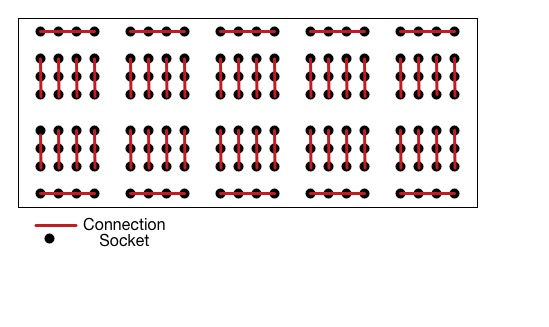
\includegraphics[scale=0.5]{Breadboard.jpg}$
    \end{center}
    \item[1.1.2] 
    \begin{center}
    $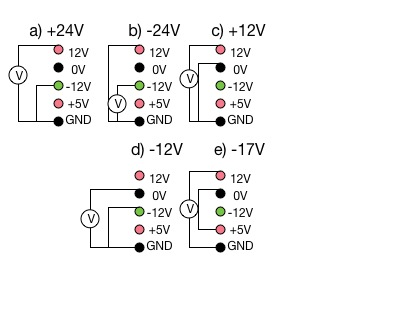
\includegraphics[scale=0.5]{powersupp.jpg}$
    \end{center}
    \item[1.1.3]
    \begin{enumerate}[label=\alph*] 
        \item 26.25 V
        \item -26.25 V
        \item 13.13 V
        \item -13.13 V
        \item 18.14 V
    \end{enumerate} 
    Not hooking up other wires yields measurement of 0.008 V when trying to measure between ground and the 12 V voltage source.\\ This happens because the 12 V does not have a common reference point, so locally, the 12V registers as approximately 0V because it has nothing to compare to. 
    \item[1.1.4] Using voltage divider equation:
    \begin{equation}
        \frac{V_A}{V} = \frac{R_2}{R_1 + R_2}
    \end{equation}
    \begin{equation}
        V_A = \frac{V*R_2}{R_1 + R_2}
    \end{equation}
    \item[1.1.5] With $V = +24V$, $R_1 = 470k$, $R_2 = 10k$, and $R_{series} = R_1 + R_2 = 470k + 10k = 480k$
    \begin{equation}
        I = \frac{V}{R_{series}} = \frac{24V}{280k} = 0.05 mA
    \end{equation}
    Note: $V$ is $V_{in}$...
    \item[1.1.6]
    \begin{equation}
        V_A = 24V * \frac{10k}{10k + 470k} = 0.5V
    \end{equation}
    \item[1.1.7] 
    \begin{enumerate}[label=\alph*]
    \item Measure current in series: 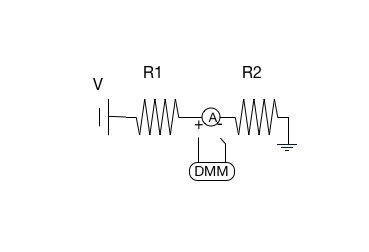
\includegraphics[scale=0.5]{Current.jpg}
    \item Measure voltage in parallel to $R_1$: 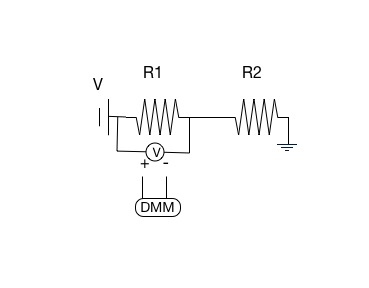
\includegraphics[scale=0.5]{Voltage.jpg}
    \end{enumerate}
    \item[1.1.8]
    We define a new function DMMErr, which gives the uncertainty in making a measurement using the Digital Multimeter (DMM):
    \begin{equation}
        DMMErr(X,Y) = 0.012\% * X + 0.004\% * Y
    \end{equation}
    where X is the measurement read on the DMM and Y is the range of the measurement; the output of DMMErr is in the units of that being measured.$R_1$ measured 470.62k $\pm$ $\Delta R_1$, $R_2$ measured 9.946k $\pm$ $\Delta R_2$, and the 24V power supply measured 26.25V $\pm \Delta V$, where $\Delta R_1$ = DMMErr(470.62k,1000k) = 0.0964744k, $\Delta R_2$ = DMMErr(9.946k,100k) = 0.000519k, and $\Delta V$ = DMMErr(26.25V,100V) = 0.00715V. \\
    The values of the resistors are well within a 5\% tolerance.
    \item[1.1.9] $I_{calculated} = \frac{5.462V}{470.62k+9.946k} \approx 5.462 * 10^{-5} A \pm \Delta I_{calculated}$ \\
    $V_A = 26.25V * \frac{9.946 k}{9.946k + 470.62k} \approx 0.5433V \pm \Delta V_A$ \\
    Where $\Delta I_{calculated}$ and $\Delta V_A$ are found from the following error functions that utilize some of the uncertainties mentioned in 1.1.8 using VMMErr and functions derived in (13) and (14):
    \begin{equation}
        \Delta I_{calculated} = \sqrt{(\frac{\partial I}{\partial V})^{2}\Delta V^{2}+(\frac{\partial I}{\partial R_1})^{2}\Delta R_1^{2}+(\frac{\partial I}{\partial R_2})^{2}\Delta R_2^{2}}
    \end{equation}
    \begin{equation}
        \Delta I_{calculated} = \frac{\sqrt{\Delta V ^{2} + (\frac{V}{R_1 + R_2})^{2}(\Delta R_1^{2} + \Delta R_2 ^{2})}}{R_1 + R_2}
    \end{equation}
    \begin{equation}
        \Delta V_A = \sqrt{(\frac{\partial V_A}{\partial V})^{2}\Delta V^{2}+(\frac{\partial V_A}{\partial R_1})^{2}\Delta R_1^{2}+(\frac{\partial V_A}{\partial R_2})^{2}\Delta R_2^{2}}
    \end{equation}
    \begin{equation}
        \Delta V_A = \frac{\sqrt{R_2^{2}\Delta V ^{2} + (\frac{V}{R_1 + R_2})^{2}(R_2^{2}\Delta R_1^{2} + R_1^{2}\Delta R_2 ^{2})}}{R_1 + R_2}
    \end{equation}
    Plugging in measured values for $V,R_1,R_2,\Delta V,\Delta R_1,\Delta R_2$ yields $\Delta I_{calculated} \approx 1.849*10^{-5} mA$ and $\Delta V_A \approx 0.00033 V$.
    \item[1.1.10] $V_A measured = 0.54291 V \pm $ VMMErr(0.54291V,1V), where the VMMErr = 0.105 mV.\\
    The uncertainty range of $V_A calculated$ from 1.1.9 is [0.54297V, 0.54363V], whereas the range for the measured value is [0.542805V,0.543015V]. The two uncertainty ranges overlap, thus the calculated and measured $V_A$ agree with each other.
    \item[1.1.11] $I_{measured} = 0.0546 mA \pm$ VMMErr(0.0546 mA, 10 mA), where the VMMErr yields an error of 0.00040655 mA. The uncertainty range for $I_{measured}$ is [0.05419V,0.05501V]. Neglecting the uncertainty range for $I_{calculated}$, and the calculated value falls well within the uncertainty range for the measured value, so the results agree.
    \item[1.1.12] 
    \begin{enumerate}[label=\alph*]
        \item From eq.(14), $I_{ideal} = 0.00005 A, R_1 = 470k\Omega,R_2 = 10k\Omega$. Using these values:
        \begin{equation}
            P_1 = I^{2}R_1 \approx 0.001175 W
        \end{equation}
        \begin{equation}
            P_2 = I^{2}R_2 \approx 2.5 * 10^{-5} W
        \end{equation}
        These powers dissipated are far less than the 0.25 W rating, so the resistors are rated for this power. 
        \item Due to the same ratio of resistance in the voltage divider, the respective voltages $V_1 = 23.5V$ and $V_2 = 0.5V$ remain the same. \\ We can express the power as:
        \begin{equation}
            P_1 = \frac{V_1^{2}}{R_1}
        \end{equation}
        \begin{equation}
            P_2 = \frac{V_2^{2}}{R_2}
        \end{equation}
        Holding $V_1$ and $V_2$ fixed, decreasing the resistor values would cause the respective power values to approach the max power rating.
        \item Setting $P_1$ and $P_2$ to max power rating 0.25 W, and exploiting $R_i = \frac{V_i^{2}}{P_i}$ yields resistance values that yield max power ratings. In this case, $R_1 max = 2209 \Omega$ and $R_2 max = 1 \Omega$. But in this case we want to see which resistor hits their max power first, keeping in mind the ratio $\frac{R_1}{R_2} = 47$. In this case $R_1$ hits its max power first, because at $R_1 max = 2209 \Omega$, $R_2 = 47 \Omega$ and still needs to decrease.
        \item $\frac{R_1 original}{R_1 max} \approx 212.765$. $R_1 max$ is about 212.765 times smaller than $R_1 max$.
    \end{enumerate}
    \item[1.1.13] See signature.
    \item[1.1.14] See signature.
    \item[1.1.15] 
        \begin{enumerate}[label=\alph*]
        \item $V_{DMM} = 5.0405V \pm 0.001005V$, the error derived from VMMErr(5.0405V,10V).
        \item $V_{Scope} = 4.97V \pm 0.67 mV$, the error found by taking the $V_{RMS}$ of the AC noise, zoomed in to 2 mV/division.
        \item $V_{Scope} = 4.97V \pm 22 mV$, the error found by taking the $V_{RMS}$ of the AC noise, zoomed in to 5 mV/division. Results between the two scope measurements are consistent, but not between them and the DMM.
        \item The fewer mV per division, more zoomed in generates more accurate results. In this case, the 2 mV/division with AC coupling option and taking the $V_{RMS}$ measurement minimizes reading error.
        \end{enumerate}
    \item[1.1.16] See signature.
    \item[1.1.17]
    \begin{equation}
        V_{RMS} = \sqrt{\frac{\int_{T_1}^{T_2}V(t)^{2}dt}{T_2 - T_1}}
    \end{equation}
    For one period T, we use the interval $t\in[0,T]$.
    \begin{enumerate}[label=\alph*]
    \item For sine wave with equation $A*sin(\frac{2\pi t}{T})$, $V_{RMS} = \sqrt{\frac{A^{2}\int_{0}^{T}sin(\frac{2\pi t}{T})^{2}dt}{T}}$ where the integral of a $sin^{2}(x)$ function over a period is $\frac{1}{2}$. This yields $V_{RMS} = A*\sqrt{\frac{1}{2}}$
    \item Using symmetry on a triangle wave function, $\frac{A*t}{T}$ for the interval $t\in[0,T]$ over period 2T, we can use eq.(25) with this interval in mind to find $V_{RMS} = \sqrt{\frac{A^{2}\int_{0}^{T}(\frac{t}{T})^{2}dt}{T}} = A\sqrt{\frac{1}{3}}$.
    \item The square wave, with value A over an interval of $T_1$ and 0 over interval of $T_2$, will have a $V_{RMS}$ over the entire period $T_1 + T_2$ of  $V_{RMS} = \sqrt{\frac{\int_{0}^{T_1}{A^{2}dt}}{T_1 + T_2}} = A \sqrt{\frac{T_1}{T_1 + T_2}}$ \\
    \end{enumerate}
    \item[1.1.18] 
        \begin{enumerate}[label=\alph*]
        \item and b, see Table 1: \begin{table}[h]
        \centering
        \caption{$V_{RMS}$}
        \label{my-label}
        \begin{tabular}{lll}
        \textbf{frequency (Hz)} & \textbf{\begin{tabular}[c]{@{}l@{}}$V_{RMS}(V)$\\ SCOPE \end{tabular}} & \textbf{\begin{tabular}[c]{@{}l@{}}$V_{RMS}(V)$\\ DMM\end{tabular}} \\
        10                      & 0.352                                                              & 0.3589                                                           \\
        20                      & 0.352                                                              & 0.3589                                                           \\
        30                      & 0.351                                                              & 0.3589                                                           \\
        50                      & 0.352                                                              & 0.3589                                                           \\
        100                     & 0.352                                                              & 0.3589                                                           \\
        300                     & 0.352                                                              & 0.3586                                                           \\
        1k                      & 0.352                                                              & 0.3583                                                           \\
        3k                      & 0.352                                                              & 0.3582                                                           \\
        10k                     & 0.353                                                              & 0.3583                                                           \\
        30k                     & 0.352                                                              & 0.3583                                                           \\
        100k                    & 0.352                                                              & 0.3581                                                           \\
        300k                    & 0.354                                                              & 0.3644                                                           \\
        500k                    & 0.355                                                              & 0.3815                                                           \\
        700k                    & 0.355                                                              & 0.4159                                                           \\
        1M                      & 0.354                                                              & 0.5105                                                          
        \end{tabular}
        \end{table}
        \item See Table 1... $V_{RMS} ideal = \frac{1V}{2\sqrt{2}}= 0.35355 V \pm 0.01768$, where the error is the 5\% tolerance and using $V_{RMS}$ of the square wave of 1.1.17, where A = 0.5V and $T_1 = T_2 = T$ such that the frequency is $f = \frac{1}{2T}$.
        \begin{center}
        $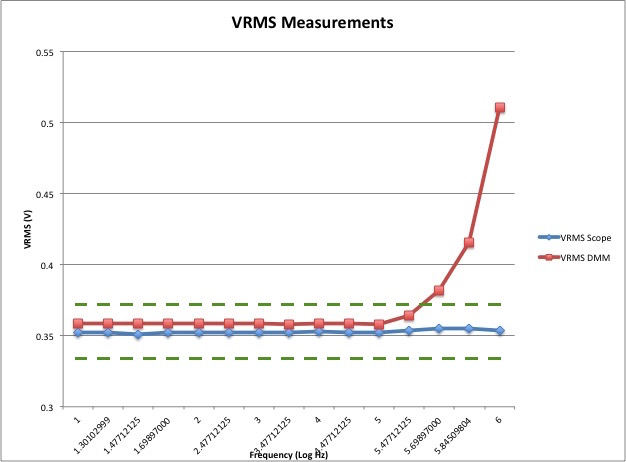
\includegraphics[scale=0.5]{VRMS.jpg}$\\
        \end{center}
        Note that the 5\% tolerance is indicated by the green dashed lines.\\
        The frequency by which DMM values are accurate lies between 10 Hz and 500kHz ($log_{10} 500k \approx 5.69$). We plot the data geometrically so we can better visualize the data in terms of order of magnitude, otherwise the data will not be evenly spaced. The DMM appears to operate within specifications, as the manual says operating limitations are between 3 Hz and 300 kHz.
    \end{enumerate}
    
    
  \item[1.1.19] See signature. 
  
\end{itemize}



\paragraph{Part 2}
\begin{itemize}
    \item[1.2.1] $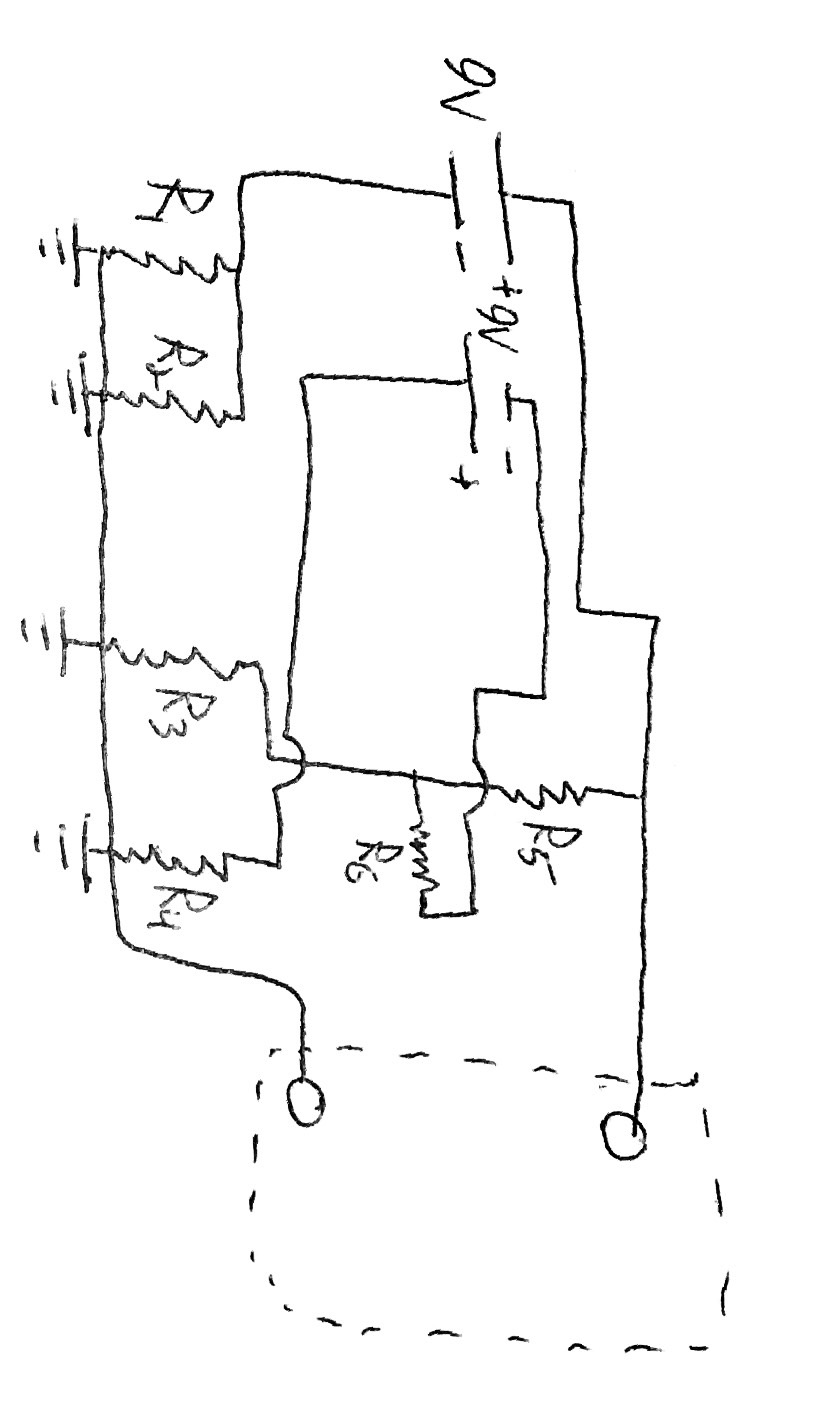
\includegraphics[scale=0.2,angle = 90]{IMG_0155.JPG}$\\ Where the following values were read off: $R_1 = 10k, R_2 = 10k, R_3 = 6.8k, R_4 = 9.1k, R_5 = 4.3k, R_6 = 2k$.\\See Table 2 for analysis of circuit... \\$ R_{th} = \frac{V_{open}}{I_{short}}$, and 
        \begin{equation}
            I_{predicted} = \frac{V_{open}-V_{out}}{R_{th}}
        \end{equation}
        \begin{center}
        $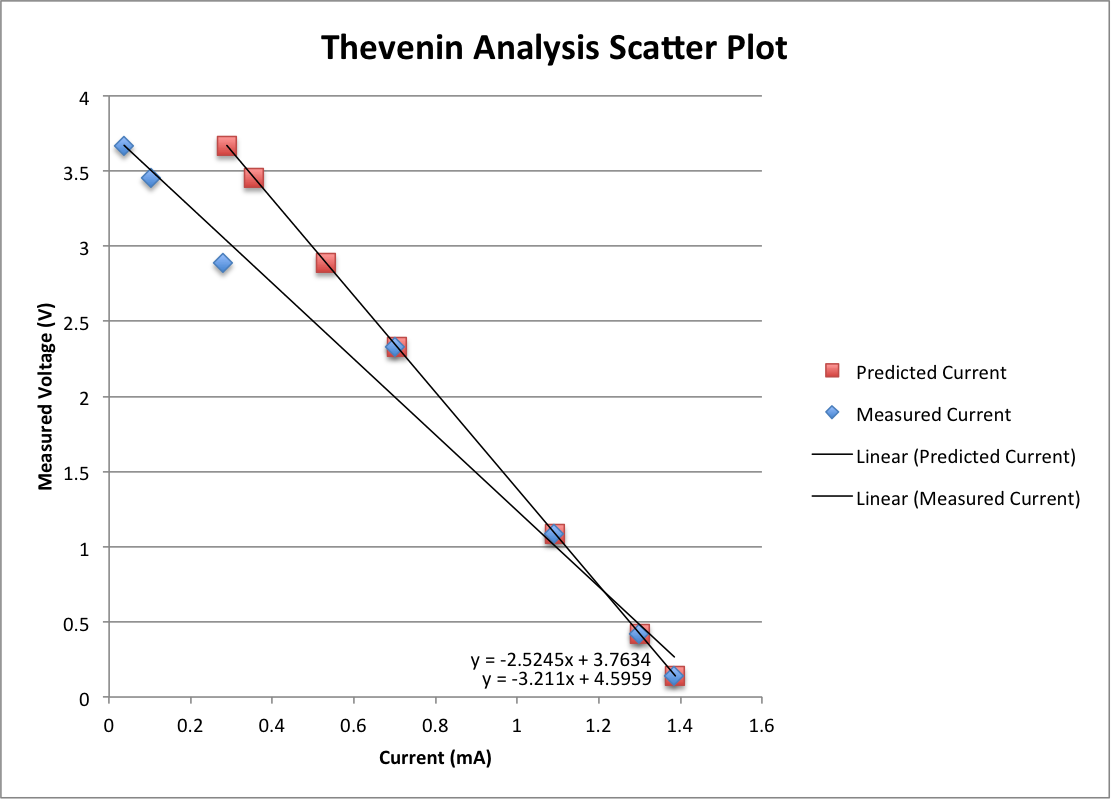
\includegraphics[scale=0.5]{ThevAnalysis.png}$\\
        \end{center}
        More or less, the thévenin circuit predicts the current values almost exactly how they were measured, except at lower current values. For the short circuit, $R_{th}$ was measured to be 3.19 k$\Omega$. Our calculated $R_{th} \approx 3.2k$. The experimental $R_{th}$ roughly corresponds with the calculated value.
        \begin{table}[h]
        \centering
        \caption{Thévenin Analysis}
        \label{my-label}
        \begin{tabular}{llll}
        R($\Omega$)               & $I_{measured} (mA)$   & $V_{measured} (V)$ & $I_{predicted} (mA)$ \\
        100             & 1.385             & 0.1408          & 1.387449393      \\
        330             & 1.298             & 0.418           & 1.301121146      \\
        1000            & 1.089             & 1.085           & 1.093397695      \\
        3300            & 0.7015            & 2.332           & 0.705045157      \\
        10000           & 0.2797            & 2.89            & 0.531267518      \\
        33000           & 0.1034            & 3.455           & 0.355309872      \\
        100000          & 0.0367            & 3.6696          & 0.28847711       \\
                        &                   &                 &                  \\
        $V_{open}$ (V) & $I_{short}$ (mA) & $R_{th}$ ($\Omega$)     &                  \\
        4.5959          & 1.4314            & 3211            &                 
        \end{tabular}
        \end{table}
    \item[1.2.2] 
    \begin{enumerate}[label=\alph*]
        \item The period of the signal appears to be around 16 ms long. This could be from the 60 Hz noise from the outlet. This is coming from the main power grid because it runs at 60 Hz.
        \item I do not see a signal if I pinch the red insulation rather than the metallic connection.
        \item I do get a clearer picture of the fuzz after playing around with it. I tried using triggering and changed my vertical divisions. The noise has peaks of different amplitudes, but has a period of roughly 20 ms. 
        \item This could be resulting from roughly 50 MHz of noise. This could come from outside interference from outside sources. Likely a lot of this noise stems from interference from the sources of the current itself, from the AC power transmission being fed into the signal generator.
    \end{enumerate}
    
    \item[1.2.3] From the voltage divider equation:
    \begin{equation}
        \frac{V}{V_{in}} = \frac{Z_{in}}{Z_{in} + R}
    \end{equation}
    \begin{equation}
        Z_{in} = \frac{V_{in}*R}{V-V_{in}}
    \end{equation}
    Where $V_{in}$ = 1V (peak to peak).\\
    Plotting $V_{out}$ versus $I$:\\
    \begin{center}
    $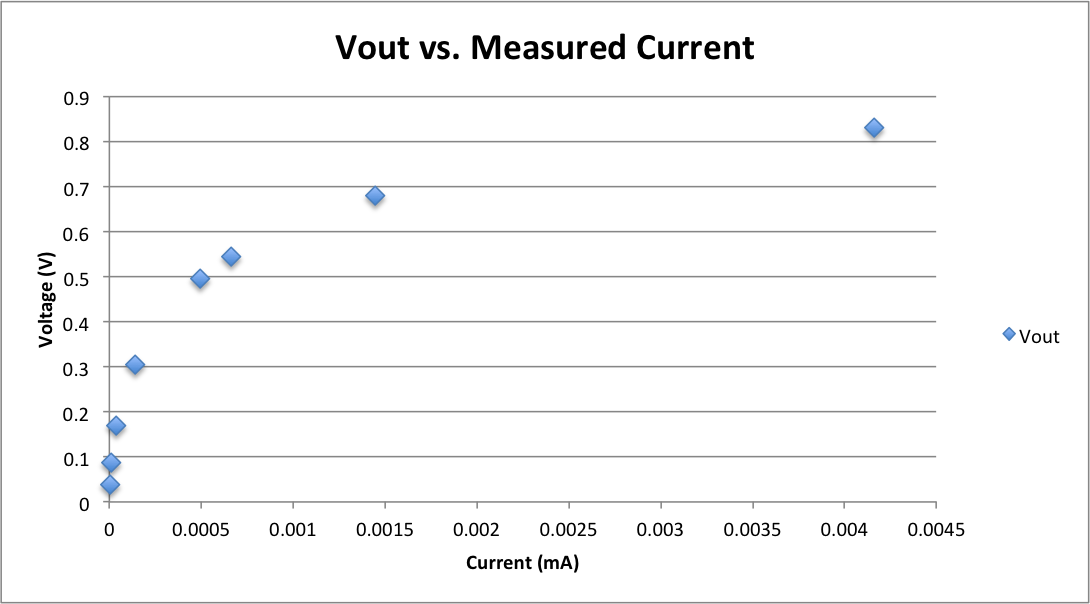
\includegraphics[scale=0.5]{1_2_3.png}$\\
    \end{center}
    From eq.(16) and from the plot, we notice that as R $\rightarrow 0$, the voltage V that we measure is the same as our input Voltage, providing us with an accurate measurement, but R $\rightarrow \infty$ will give us an extremely low and nearly zero value of measured $V$. We would expect there to be a linear dependence of $V_{in} = I_{in}Z_{in}$. However, the data in the plot above appears to show nonlinear dependence with the introduction of the load R. Generating a best fit model and taking the derivative of the model yields a function of the input impedance. A best fit logarithmic model yields $V_{model} = 0.1063ln(I) + 1.3355$ with correlational $R^{2} = 0.94322$. The partial derivative of $V_{model}$ with respect to I yields $Z_{in} = \frac{0.1063Volts}{I} k\Omega$ with units of mA for I. Using the $R^{2}$, we estimate uncertainty to be about 6\%.\\ The data can be found in the following table 3:
    \begin{table}[h]
    \centering
    \caption{$V_{out} vs I$}
    \label{my-label}
    \begin{tabular}{llll}
    \textbf{R ($\Omega$)} & \textbf{V (V)} & \textbf{I out (mA)} & \textbf{Actual Z in ($\Omega$)} \\ \hline
    0                     & 1              & infinity            & infinity                        \\
    200000                & 0.832          & 0.00416             & 990476.1905                     \\
    470000                & 0.68           & 0.001446809         & 998750                          \\
    820000                & 0.544          & 0.000663415         & 978245.614                      \\
    1000000               & 0.496          & 0.000496            & 984126.9841                     \\
    2200000               & 0.304          & 0.000138182         & 960919.5402                     \\
    4700000               & 0.169          & 3.59574E-05         & 955836.3418                     \\
    10000000              & 0.088          & 0.0000088           & 964912.281                      \\
    20000000              & 0.0384         & 0.00000192          & 798668.8852                    
    \end{tabular}
    \end{table} \\Where V is $V_{out}$

    
    \item[1.2.4] See table 4:\\
    \begin{table}[h]
    \centering
    \caption{$V_{out} vs I$ using Scope Probe}
    \label{my-label}
    \begin{tabular}{llll}
    \textbf{R ($\Omega$)} & \textbf{V (V)} & \textbf{Iout (mA)} & \textbf{Actual Zin ($\Omega$)} \\ \hline
    0                     & 0.98           & infinity           & 0                              \\
    820000                & 0.9            & 0.001097561        & 7380000                        \\
    1000000               & 0.9            & 0.0009             & 9000000                        \\
    2200000               & 0.8            & 0.000363636        & 8800000                        \\
    4700000               & 0.66           & 0.000140426        & 9123529.412                    \\
    10000000              & 0.496          & 0.0000496          & 9841269.841                    \\
    20000000              & 0.296          & 0.0000148          & 8409090.909                   
    \end{tabular}
    \end{table}\\ Using the same calculations from 1.1.3, besides R=0, the scope probe appears to have a higher input impedance measured than with the scope alone by a factor of around 10.
    
    
    \item[1.2.5] See Table 5... Please ignore both $\Delta$
    $Z_{out}$s as they reflect only two data points to ascertain output impedance. The output impedance was found for both setting levels by taking the negative of the slope of a linear regression of the I vs. $V_{out}$ data set. This yields a $Z_{out}$ of 48.031 $\Omega$ for the 50 $\Omega$ Setting and a $Z_{out}$ of 53.47 $\Omega$ for the high Z setting, with $R^{2}$ correlational values of 0.995 and 0.992 respectively.

        \begin{table}[h]
        \centering
        \caption{Output Impedance}
        \label{my-label}
        \begin{tabular}{cccc}
                      & \textbf{50$\Omega$ Setting}    & \textbf{High Z Setting} & \textbf{50$\Omega$ Setting}    \\ \cline{2-4} 
        \textbf{R($\Omega$)} & \textbf{Vout(mV)}       & \textbf{Vout(mV)}       & \textbf{I (mA)}         \\
        3             & 60                      & 25.2                    & 20                      \\
        10            & 162                     & 81                      & 16.2                    \\
        33            & 404                     & 196                     & 12.24242424             \\
        100           & 665                     & 332                     & 6.65                    \\
        330           & 860                     & 436                     & 2.606060606             \\
        1000          & 950                     & 460                     & 0.95                    \\
                      & \textbf{High Z Setting} & \textbf{50 $\Omega$ Setting}    & \textbf{High Z Setting} \\ \cline{2-4} 
        \textbf{R($\Omega$)}    & \textbf{I (mA)}         & \textbf{$\Delta$Zout(Ignore)($\Omega$)}         & \textbf{$\Delta$Zout(Ignore)($\Omega$)}        \\
        3             & 8.4                     & n/a                     & n/a                     \\
        10            & 8.1                     & 26.84210526             & 186                     \\
        33            & 5.939393939             & 61.14854518             & 53.22580645             \\
        100           & 3.32                    & 46.67027906             & 51.92040722             \\
        330           & 1.321212121             & 48.22030723             & 52.03153426             \\
        1000          & 0.46                    & 54.34583715             & 27.8676988             
        \end{tabular}
        \end{table}
    \item[1.2.6]
    $R_{ideal} = 100k$, $C_{ideal} = 10 nF$, $R_{measured}= 99.7 \pm 0.4 k$, $C_{measured} = 9.99 \pm 2 nF$ \\  From [1.2.6], after setting up the proper configuration, we attained the following image on our oscilloscope: \\
    \begin{center}
    $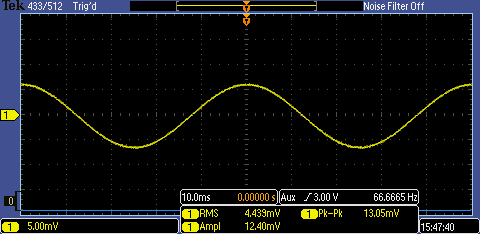
\includegraphics[scale=0.5]{TEK00000.PNG}$
    \end{center}
    
    \item[1.2.7] See Table 6 for measurements... In the graph below, the rolloff point for the transfer function output is labelled as a yellow diamond. To produce the data, $V_{in}$ is 0.5V, $V{RMS}$ for a sine signal was measured, and the following relationships were utilized:\\
    \begin{equation}
        V_{out} = \sqrt{2}V_{RMS}
    \end{equation}
    And for rolloff frequency, where $\frac{V_{in}}{V_{out}} = \frac{1}{\sqrt{2}}$, we needed to measure $V_{RMS}$ of
    \begin{equation}
        V_{RMS}rolloff = \frac{V_{out}}{\sqrt{2}} = \frac{V_{in}}{2} = 0.25V
    \end{equation}
    We use $\frac{V_{out}}{V_{in}} = \frac{1}{\sqrt{2}}$ instead of $\frac{1}{2}$ for many reasons. At such a value, the output power is one half of its original,the point is an "inflection" point of the transfer function graph, and it is used to derive the $f_{3dB}$ frequency. For bandpass circuits, the range of frequencies that lie between two of such points define the bandwidth of a signal, which has many practical applications.\\
    \begin{center}
    $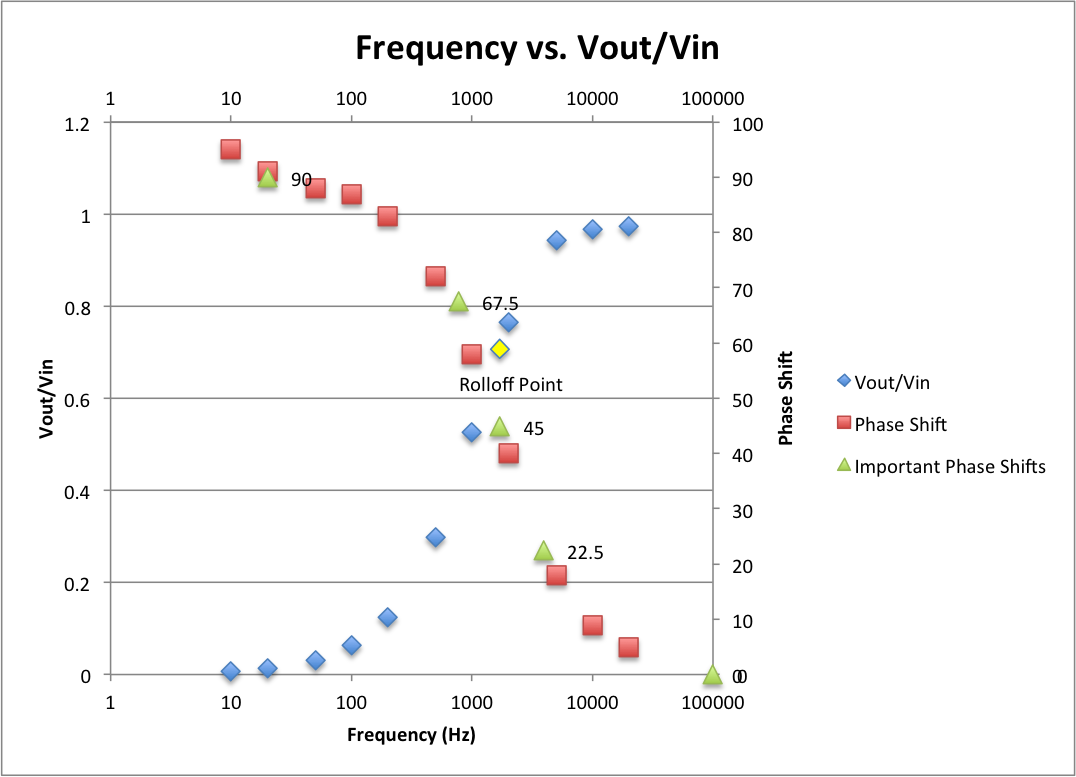
\includegraphics[scale=0.6]{1_2_7.png}$
    \end{center}
    \begin{table}[h]
    \centering
    \caption{Transfer function and Phase Shift for Given Frequency}
    \label{my-label}
    \begin{tabular}{ccccc}
    \multicolumn{1}{l}{\textbf{Frequency (Hz)}} & \multicolumn{1}{l}{\textbf{Vrms (mV)}} & \multicolumn{1}{l}{\textbf{Vout (mV)}} & \multicolumn{1}{l}{\textbf{Vout/Vin}} & \multicolumn{1}{l}{\textbf{Phase Shift ($\degree$)}} \\ \hline
    10                                          & 2.184                                  & 3.08864242                             & 0.006177285                           & 95                                         \\
    20                                          & 4.41                                   & 6.23668181                             & 0.012473364                           & 91                                         \\
    50                                          & 11.05                                  & 15.62705986                            & 0.03125412                            & 88                                         \\
    100                                         & 22.13                                  & 31.29654614                            & 0.062593092                           & 87                                         \\
    200                                         & 43.57                                  & 61.61728491                            & 0.12323457                            & 83                                         \\
    500                                         & 105                                    & 148.492424                             & 0.296984848                           & 72                                         \\
    1000                                        & 185.9                                  & 262.9023012                            & 0.525804602                           & 58                                         \\
    2000                                        & 270.4                                  & 382.4033473                            & 0.764806695                           & 40                                         \\
    5000                                        & 333.7                                  & 471.9230658                            & 0.943846132                           & 18                                         \\
    10000                                       & 342.2                                  & 483.943881                             & 0.967887762                           & 9                                          \\
    20000                                       & 344.5                                  & 487.1965722                            & 0.974393144                           & 5                                          \\
    20                                          &                                        &                                        &                                       & 90                                         \\
    770                                         &                                        &                                        &                                       & 67.5                                       \\
    1700 (rolloff)                                        &                         $\sim$ 250              &                                        &     $\frac{1}{\sqrt{2}}$ (rolloff)                                  & 45 (rolloff)                                         \\
    3900                                        &                                        &                                        &                                       & 22.5                                       \\
    100000                  &                   &                    &                 & 0                  
    \end{tabular}
    \end{table}
    
    \item[1.2.8] See Table 6 and the graph of [1.2.7] for corresponding measurements of frequency vs phase shift. The points detailing the $0\degree,22.5\degree,45\degree,67.5\degree,90\degree$ phase shifts are labelled in green. Notice how the 45$\degree$ point is at the same frequency as the $\frac{V_{out}}{V_{in}}$ rolloff points. Thus, there is a rolloff point at 45$\degree$. Note how the absolute value of the phase shift has been taken in the plot above.
    
    \item[1.2.9 Analysis:]  We can calculate our predicted transfer function and phase angle through the following analysis, using R = 100k, C = 10 nF and j = $\sqrt{-1}$:\\
    \begin{equation}
        Z_{tot} = R + Z_C = R - \frac{j}{\omega C}
    \end{equation}
    The predicted phase angle ($\phi$) can be found by:
    \begin{equation}
        tan(\phi) = \frac{\frac{-1}{\omega C}}{R}
    \end{equation}
    To which:
    \begin{equation}
        \phi = tan^{-1}(-\frac{1}{2\pi f R C})
    \end{equation}
    As for the transfer function:
    \begin{equation}
        |H(\omega)| = |\frac{V_{out}}{V_{in}}| = |\frac{R}{R+X_C}| = |\frac{R}{R-\frac{j}{\omega C}}| = \frac{R}{\sqrt{R^{2} + (\frac{1}{2\pi f C})^{2}}}
    \end{equation}
    Plotting the results found in [1.2.8] versus the predicted results found in eq.(20)-(23) and including the measured gain $G = 20 log_{10} |\frac{V_{out}}{V_{in}}|$, and taking the absolute values of phase shifts and the transfer funtion yields:\\ 
    \begin{center}
    $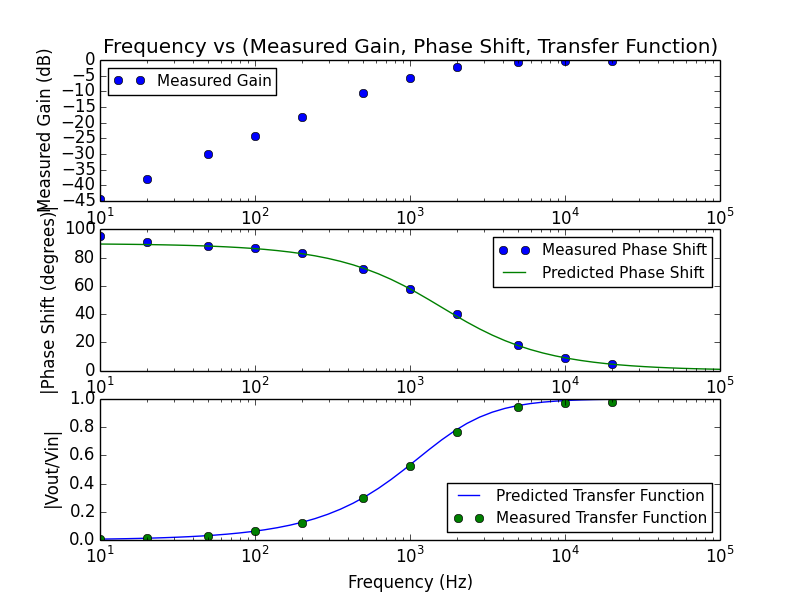
\includegraphics[scale=0.6]{plotRCGain.png}$
    \end{center}
    Most certainly, the rolloff points between the predicted/theoretical and measured/experimental plots agree, as evidenced by the closeness of fit of the plots.
    
    \item[1.2.9 Bandpass:] 
        Design:\\
        \begin{center}
        $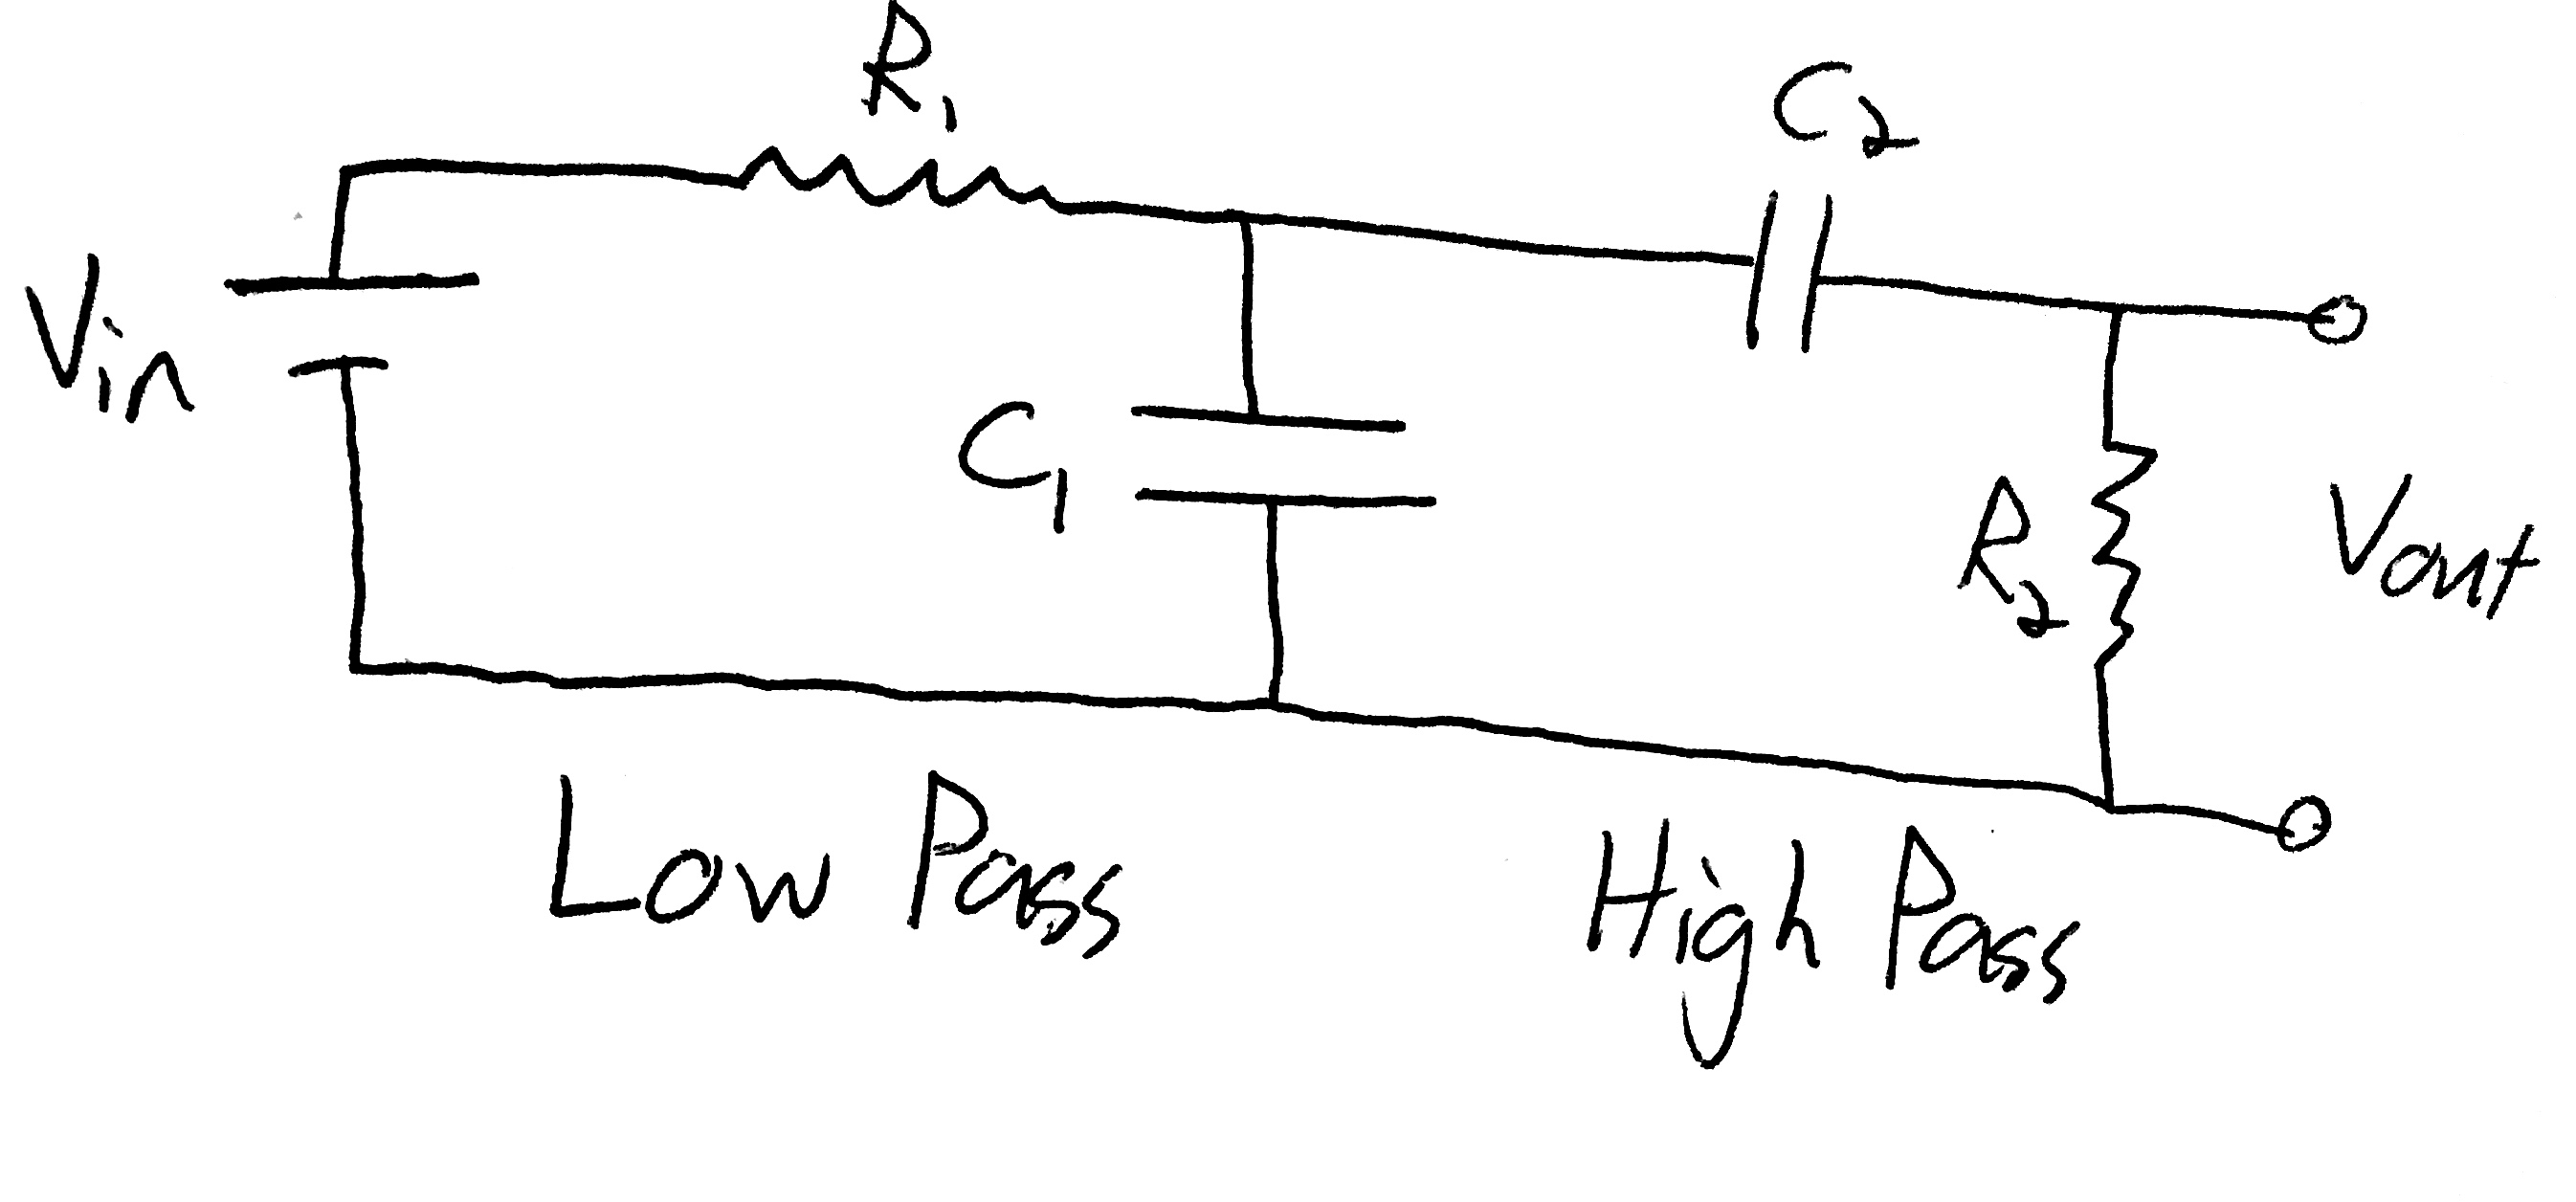
\includegraphics[scale=0.1]{IMG_0149.JPG}$\\
        \end{center}
        The bandpass filter was built using a low pass filter in series with a high pass filter, as evidenced by the drawing. In this case, the low pass is in the upper leg, and the high pass in the lower leg of the circuit. $R_1$ was chosen to be 100$\Omega$ and $R_2$ was chosen to be 100k in the design. We utilizing the formula for the rolloff points for each filter using rolloff frequencies $f_1$ = 10kHz for the low pass and $f_2$ = 500 Hz for the high pass:\\
        \begin{equation}
            f_{3dB} = \frac{1}{2\pi R C}
        \end{equation}
        To find that $C_1$ should be:\\
        \begin{equation}
            C_1 = \frac{1}{2\pi R_1 f_1} \approx 200 nF
        \end{equation}
        and $C_2$:\\
        \begin{equation}
            C_2 = \frac{1}{2\pi R_2 f_2} \approx 3 nF
        \end{equation}
        Prior to integrating them into the circuit, we measured that $R_1 = 99.3 \pm 0.015916\Omega$, $R_2 = 99.2 \pm 0.015904k\Omega$, $C_1 = 97.3 \pm 0.3 nF$ (could not find 200 nF capacitor) and $C_2 = 3.24 \pm 0.4 nF$. $R_1$ and $R_2$ errors found from VMMErr equation.\\ The maximum voltage we were able to measure using proper impedance loading practices was $V_{max} = 913mV$ @ a frequency of 2kHz. Thus, we'd expect to find our rolloff points at a $V_{out}rolloff = \frac{V_{max}}{\sqrt{2}} \approx 646 mV$. The rolloff points will be illuminated in the plot, and are the yellow data points. As depicted in Table 7, the rolloff points at frequencies of 470 Hz and 11300 Hz roughly correspond to the original rolloff points (500 Hz and 10 kHz) in question.\\
        \begin{center}
        $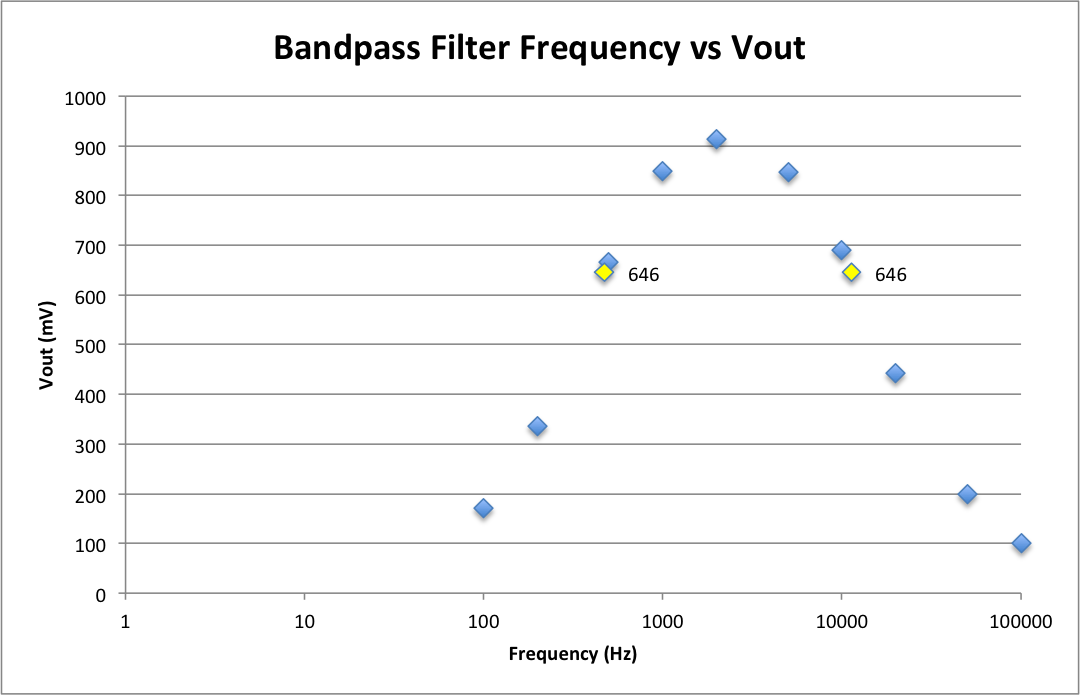
\includegraphics[scale=0.6]{1_2_9.png}$\\
        \end{center}
        \begin{table}[h]
        \centering
        \caption{Bandpass Filter Data}
        \label{my-label}
        \begin{tabular}{ccc}
        \textbf{Frequency (Hz)} & \textbf{Vout (mV)} &                \\ \cline{1-2}
        100                     & 170                &                \\
        200                     & 336                &                \\
        500                     & 665                &                \\
        1000                    & 850                &                \\
        2000                    & 913                &                \\
        5000                    & 848                &                \\
        10000                   & 691                &                \\
        20000                   & 442                &                \\
        50000                   & 200                &                \\
        100000                  & 101                &                \\
        11300                   & 646                & $\leftarrow$ Rolloff Point! \\
        470                     & 646                & $\leftarrow$ Rolloff Point!
        \end{tabular}
        \end{table}
        \item[1.2.10] 
            \begin{enumerate}[label = \alph*]
                \item \begin{center} $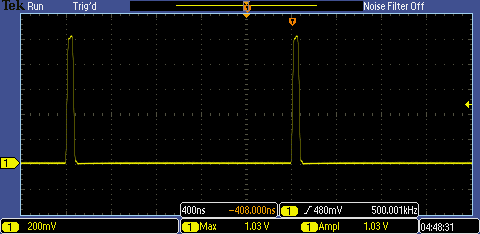
\includegraphics[scale=0.4]{a1.PNG}$\end{center}
                \item The signal is reduced/suppressed after adding the terminator:\\\begin{center} $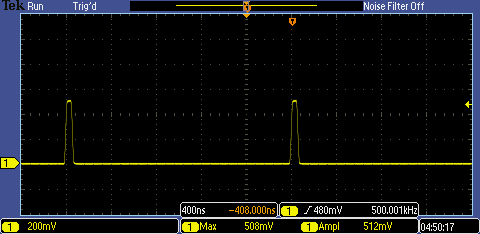
\includegraphics[scale=0.4]{b1.PNG}$\end{center} 
                 The signal disappears after adding the short:\\
                \begin{center} $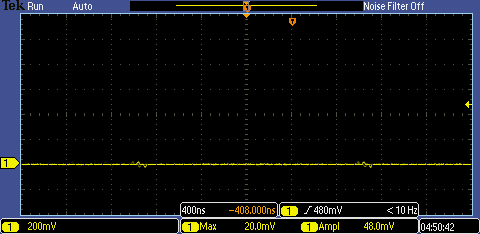
\includegraphics[scale=0.4]{b2.PNG}$\end{center}
                \item \begin{center} $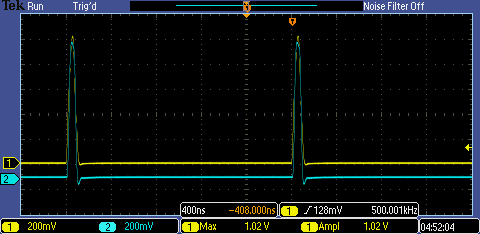
\includegraphics[scale=0.4]{c1.PNG}$\end{center}
                After replacing BNC with 100ft cable, I am surprised, as there appear to be multiple reflections of the signal:\\
                \begin{center} $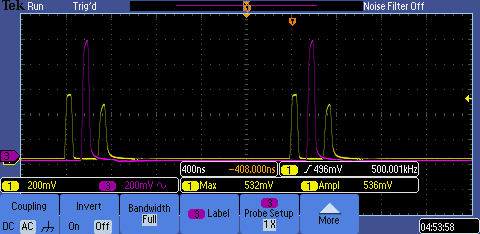
\includegraphics[scale=0.4]{c2.PNG}$\end{center}
                Adding the terminator gets suppresses the signal of the reflections and decreases the amplitude:\\
                \begin{center} $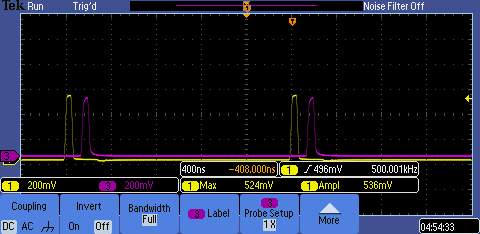
\includegraphics[scale=0.4]{c3.PNG}$\end{center}
                The signal at the far end is delayed relative to the signal at the near end because the delay is the amount of time it takes for light to travel through the medium between the two ends:\\
                \begin{center} $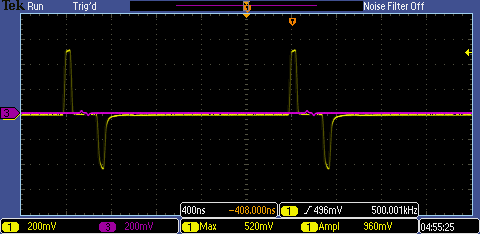
\includegraphics[scale=0.4]{c4.PNG}$\end{center}
                The upright signals reflect the signal travelling from an electrically dense region to a more rarefied region, and the upside down signals demonstrate signals travelling from a rarefied region to a denser region.
                \item Series resistance: Normal: The far and near end has signals of multiple reflections of decreasing amplitude.\\ \begin{center} $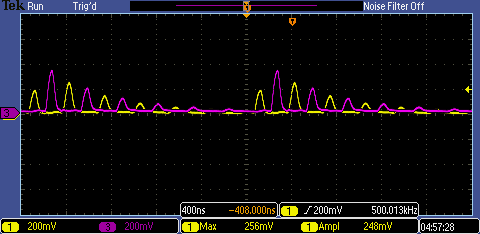
\includegraphics[scale=0.4]{d1.PNG}$\end{center}
                Terminator: All reflected signals are suppressed and the far end signal has  amplitude as large as near end.\\
                \begin{center} $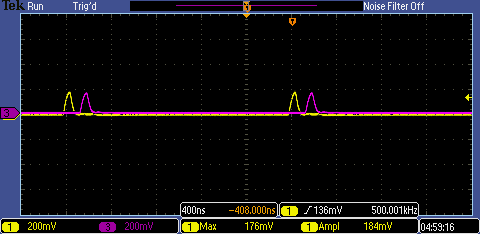
\includegraphics[scale=0.4]{d2.PNG}$\end{center}
                Shorted: All signals from the far end are eliminated, with the near end seeing upside down and right side up reflections.\\
                \begin{center} $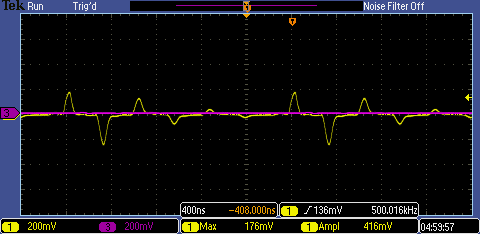
\includegraphics[scale=0.4]{d3.PNG}$\end{center}
                \item Parallel resistance: Normal: Far end has reoccurring pattern of reflections, first one being upside down, second right side up, with decreasing amplitude.\\ \begin{center} $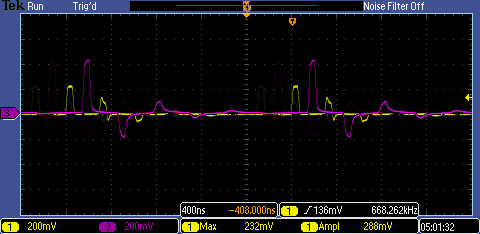
\includegraphics[scale=0.4]{e1.PNG}$\end{center}
                Terminator: Reflections suppressed once again.\\
                \begin{center} $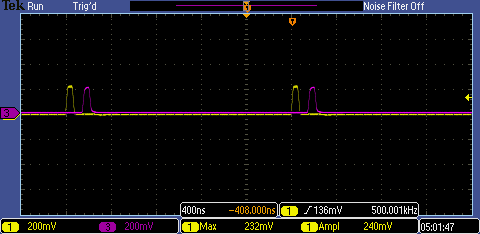
\includegraphics[scale=0.4]{e2.PNG}$\end{center}
                Shorted: Far end signal eliminated and the near end has its signal reflected upside down.\\
                \begin{center} $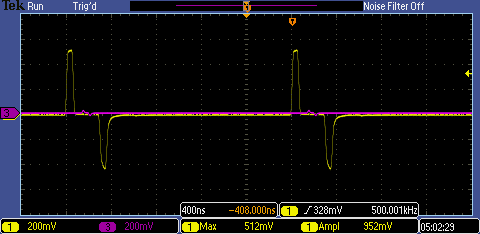
\includegraphics[scale=0.4]{e3.PNG}$\end{center}
                Expected results came with use of terminator, extraneous signals come from normal usage, and getting some upside down signals from the short. Parallel resistance normal usage also generates upside down signals.
                \item I placed a 300$\Omega$ terminator/parallel resistor in the far end in order to obtain a clean signal. \\Before:\\ \begin{center} $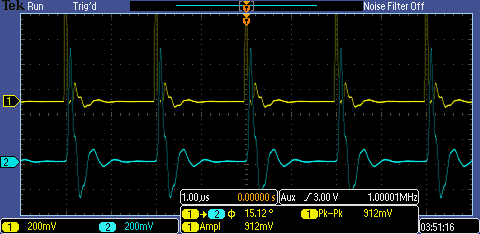
\includegraphics[scale=0.4]{f1.PNG}$ \end{center}
                 After:\\
                \begin{center} $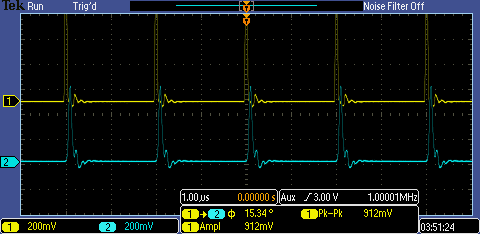
\includegraphics[scale=0.4]{f2.PNG}$\\\end{center} The 300$\Omega$ coaxial cable is impedance matched with the 300 $\Omega$ resistor, and this matching suppresses reflections upon a further Maxwell analysis. It increases the $Z_{in}$ of the oscilloscope.
                
            \end{enumerate}
            
    \item[1.2.11] Speed of light, c, is $\approx$ 300,000km/s. Consider speed of signal through cable, $c_n = \frac{2 c}{3} \approx 200000 km/s$. Taking a look into [1.2.10e] for the shorted system, we see that there is $\sim$ 340 ns delay between the beginning of the near end pulse and the beginning of its reflection. This is the time it took for the signal to travel through the ($100ft = 30.48m$) coaxial cable and reflect and come back.\\ Now, finding the time it takes for a signal travelling at $c_n$ to travel to end and back of 100 ft coaxial cable, and we find:
    \begin{equation}
        t = \frac{2*100ft}{c_n} = \frac{2*30.48m}{2*10^{8} m/s} \approx 304 ns
    \end{equation}
    The value for the time light takes to travel through a 100ft coaxial cable and back is nearly the same as the time measured of the reflected pulse. This accounts for our measurements. We see extra pulses on the near end because the extra signals are reflected backwards from the large BNC/coaxial cable. The extra pulses are reflections as light travels to a denser or rarefied medium. As signals pass boundaries from low to higher impedance medium, upside down reflections are produced with 180 degree phase shifts. As signals pass from high to low mediums, no phase change is noticed upon reflection (right side up) Sometimes the pulses are not there at all because of impedance matching at the boundaries.
    
    \item[1.2.12] 
    For the "no load" output, we know that $V_{out}$ = $V_{th}$. Now, this output is reduced by 20\% as we add a load, R, of 1k$\Omega$; that is, $V_{out new} = 0.8*V_{th}$. We are given the new voltage divider equation, $\frac{V_{out new}}{V_{th}} = \frac{R}{Z_{out} + R}$. Plugging in the above values, and we get:
    \begin{equation}
        0.8 = \frac{1k\Omega}{Z + 1k\Omega}
    \end{equation}
    \begin{equation}
        Z*(0.8) + 0.8k = 1k
    \end{equation}
    To which we find that $Z_{out}$ = 250 $\Omega$.
    
    \item[1.2.13]  Using the power equation, we find that the expected dissipative power of the light bulb is:
    \begin{equation}
        P = \frac{V^{2}}{R} = \frac{(110V)^{2}}{9\Omega} \approx 1344.44 W
    \end{equation}
    This is certainly not the amount of power that we'd expect the 100W light bulb to use. The 100W power number is right here, else the 1344 watt power output will likely ruin circuit elements or cause burn out. The light bulb is a nonlinear circuit element in that the increasing temperature of the tungsten (or whatever element is being heated) is increasing the resistance of the light bulb which in turn reduces power to safer levels. The increasing resistance due to temperature and other factors causes the power output to reduce to safer levels.
        
\end{itemize}

\section{Signatures}
\centering
$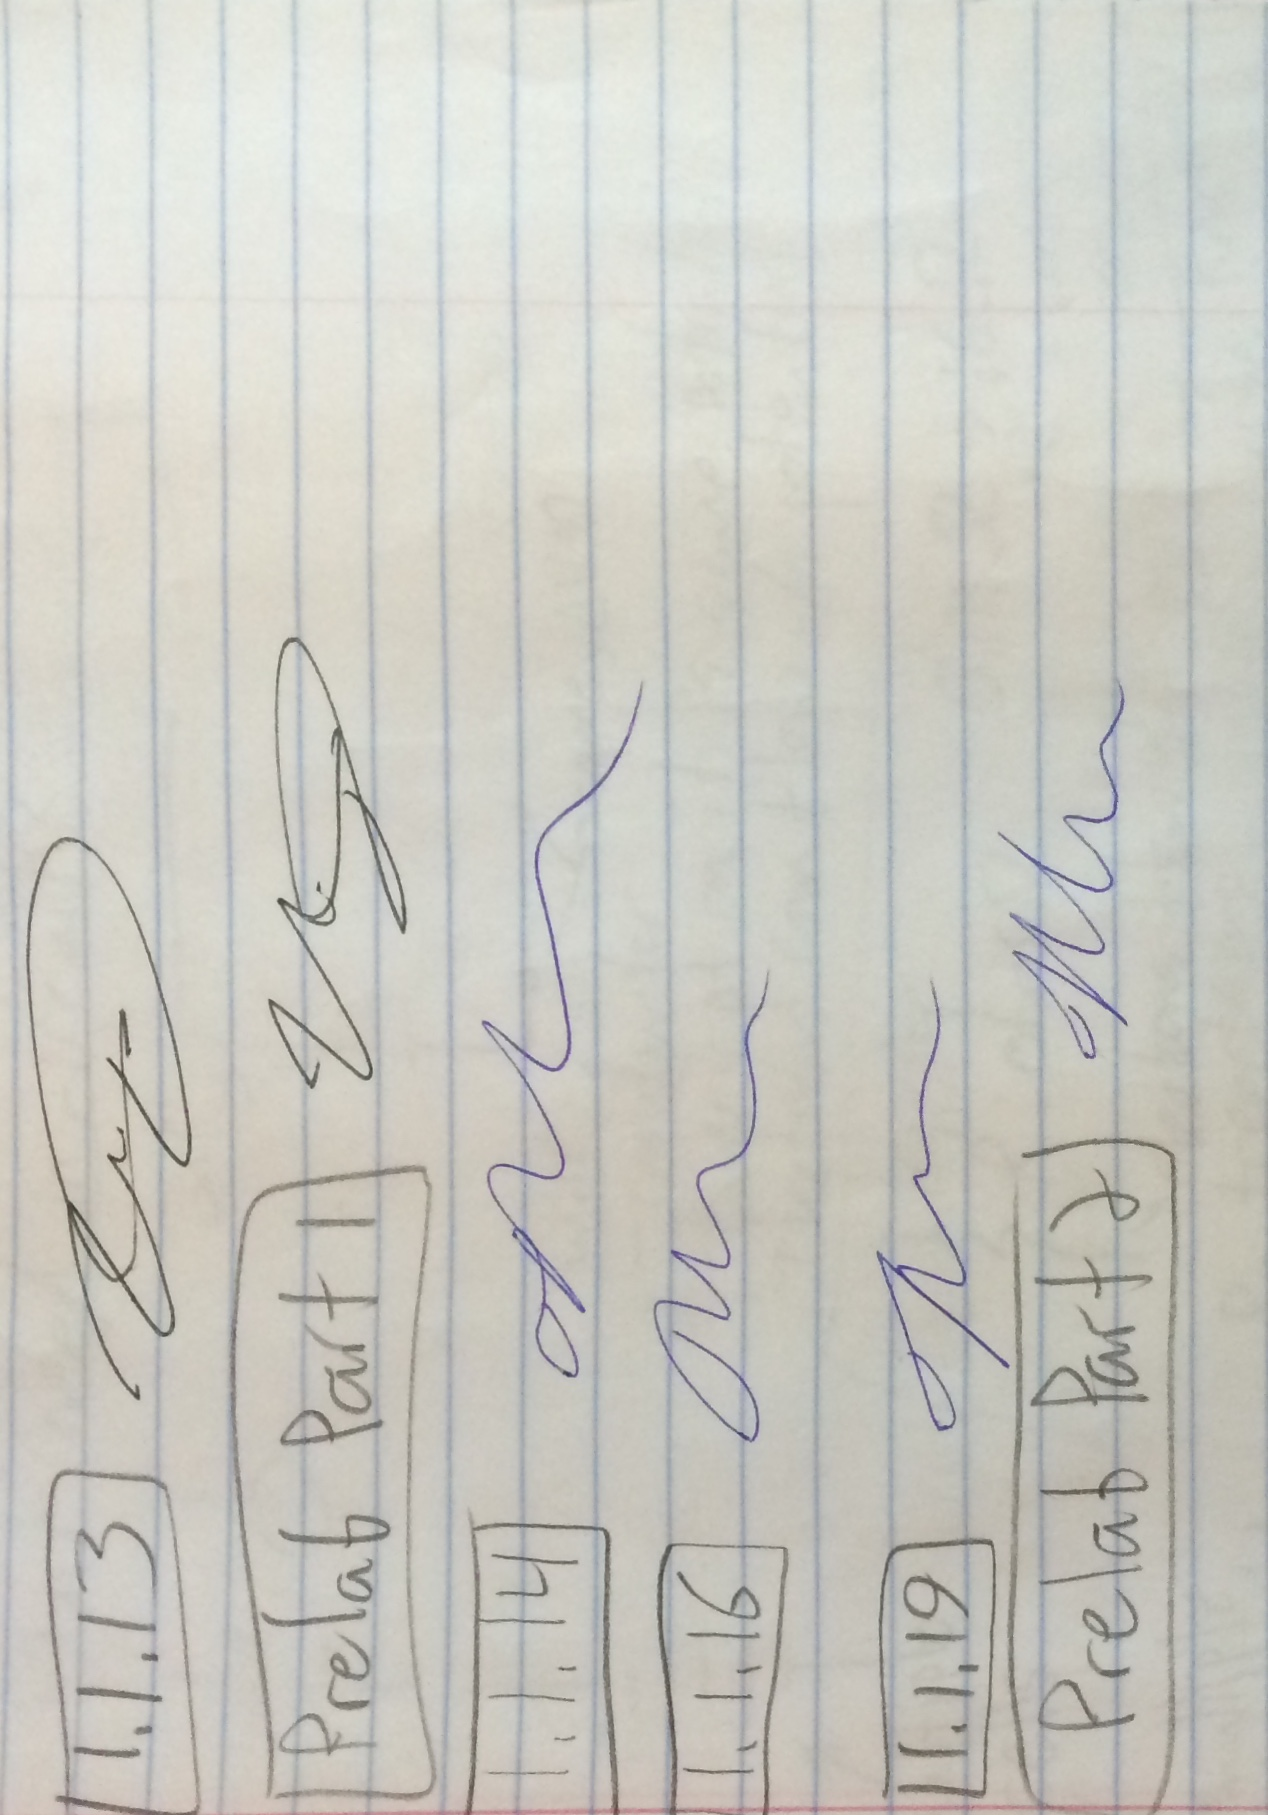
\includegraphics[angle = -90,scale = 0.2]{IMG_0137.JPG}$



Stuff left to do... Cite Sources for f3dB, 1.2.1, 

\end{document}
